% !TEX root = ../thesis.tex

\chapter{Analýza}

Analýza sa bude zaoberať dátami využiteľnými pri implementácii umelej inteligencie a zároveň analýze hier a ich využití.

\section{Analýza potenciálnych počítačových hier}
Bližšie si pozrieme kandidátov hier na základe možností dát, produktivity, veľkosti ich publika a investovaných fondov do tipovania.

\subsection{Counter-Strike: Global Offensive}
Hra s priemerným publikom viac ako 500 000 hráčov každý deň, publikovaná v roku 2012.\cite{csgoplayers} Práve prebieha svetový šampionát vo Švédsku s výherným rozpočtom 2 miliónov dolárov. Veľkou časťou tejto hry je verejne dostupný trh s predmetmi získateľnými iba cez túto hru. Tieto predmety majú na podobnom základe ako NFT´s peňažnú hodnotu a poskytujú hráčom vsadiť cez tretie strany na výhercov konkrétnych zápasov, čo viacnásobne zväčšuje tipovací trh. Problémom pri FPS hrách je ale určenie potrebných dát na predpoveď. Výsledok má príliš veľa variácií, kde len milimetre rozhodujú o úplnej zmene priebehu. Dalo by sa určiť víťaza na základe predošlých stretnutí daných dvoch tímov, no tímy sú veľmi ovplyvnené zmenami hráčov, ktoré môžu úplne zmeniť tímovú atmosféru a dáta z predošlých hier sú irelevantné.

 \subsubsection{Predpovede počas zápasu}
 Jedna hra sa delí na 30 kôl. Prvý tím, ktorý dosiahne 16 bodov, vyhráva. Počas kola už firma Valve, tvorca tejto hry, ukázala ich prieskumy a ukazuje, aká je šanca, že daný tím vyhraje kolo na základe miliárd kôl z predchádzajúcich hier. Percentá sa menia podľa počtu živých hráčov, počtu peňazí, mapy, strany a položenia bomby. Za túto funkciu som musel zaplatiť 0,85 eur za mesiac.


  
 \begin{figure}[h!]
 
 	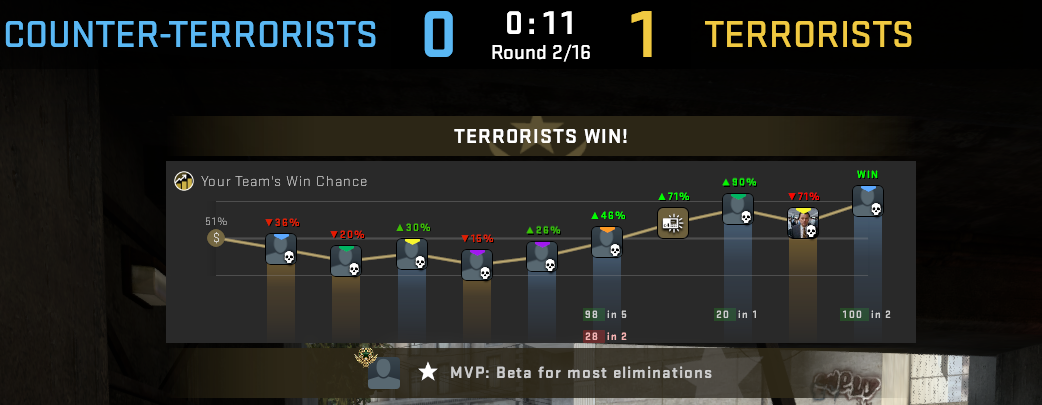
\includegraphics[width=.9\textwidth]{figures/jednanula}
 	\centering
 	\caption{\LaTeX{} Na začiatku môžeme vidieť 51 percentnú pravdepodobnosť na výhru, pri prvom úmrtí nášho spoluhráča šanca klesla na 36 percent, pri druhom až na 20, ale pri zabití nepriateľa šanca stúpla na 30 percent.  \label{jednanula}}
 \end{figure}

  \begin{figure}[h!]
  	
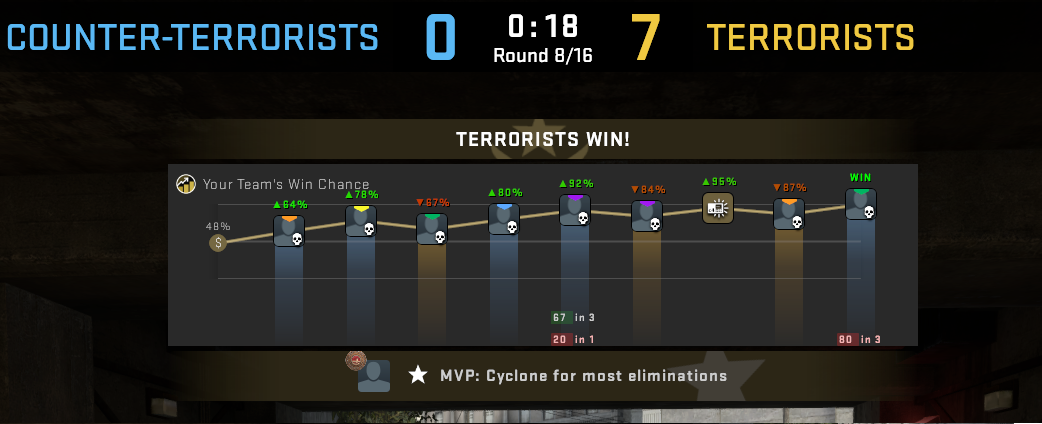
\includegraphics[width=.9\textwidth]{figures/sedemnula}
\centering
\caption{\LaTeX{} Vieme vydedukovať, že čím je šanca na výhru vyššia, tým sa šanca na úmrtie spoluhráča takisto zmenšuje. 
\label{sedemnula}}
\end{figure}

\begin{figure}[h!]
	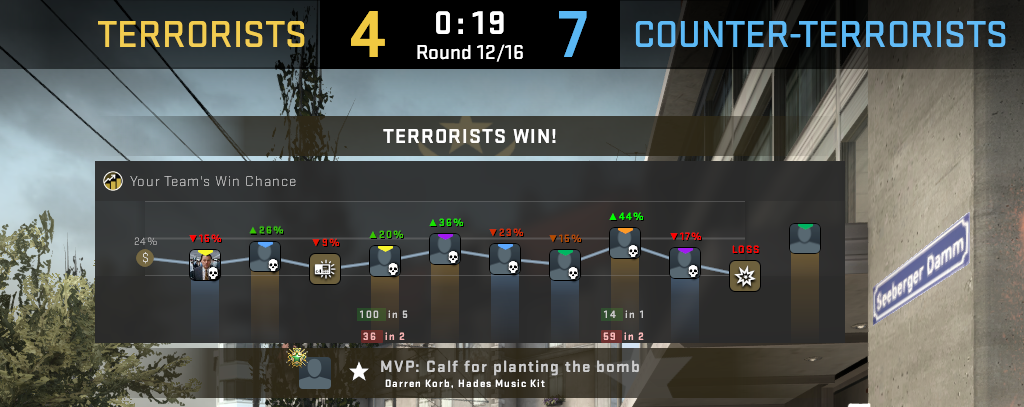
\includegraphics[width=.9\textwidth]{figures/sedemstyri}
	\centering
	\caption{\LaTeX{} Hneď prvé percento je veľmi nízke, len 24 percent, a to kvôli horšiemu vybaveniu/peňažnej situácie nášho tímu.
		\label{sedemstyri}}
\end{figure}

\begin{figure}[h!]
	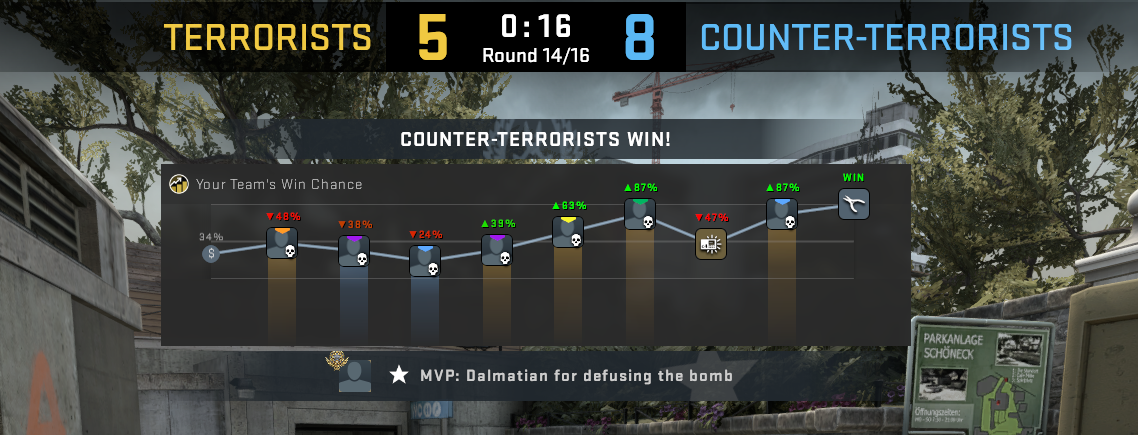
\includegraphics[width=.9\textwidth]{figures/osempat}
	\centering
	\caption{\LaTeX{} Z prvého prechodu si môžete všimnúť stúpnutie šance z 34 na 48 percent, aj keď bol zabitý jeden z našich spoluhráčov. 
		\label{osempat}}
\end{figure}

\subsubsection{Potrebné dáta hry Counter-Strike: Global Offensive :}

 
 PlayerId - unikátne ID hráča \\
 Name - meno hráča \\
 TeamId - unikátne meno tímu hráča \\
 Team - meno tímu hráča \\
 Opponent - meno opozičného tímu \\
 DateTime - čas zápasu \\
 OpponentId - ID opozičného tímu \\
 Games - počet hraných hier\\
 Maps - počet hraných máp\\
 Kills - počet zabití\\
 Assists - počet asistencií\\
 Deaths - počet smrtí\\
 Headshots - počet zabití streľbou do hlavy\\
 AverageDamagePerRound - priemerné poškodenie za kolo\\
 EntryKills - počet hráč mal prvé zabitie v kole\\
 Winner - víťaz

 

 \subsubsection{Vyhodnotenie Counter-Strike: Global Offensive}
 Pri vyhodnocovaní použiteľnosti hry sme sa pozerali na 3 oblasti. \\ \\ Potenciál/veľkosť publika a stávkovania. Efektívnosť využitia umelej inteligencie. Dostupnosť, respektíve využiteľnosť dát z hier. \\ \\
 Z hľadiska obecenstva, dostupnosti a možnosti stávkovania je CSGO veľmi lukratívna možnosť. Databáza hráčov je rozsiahla nielen v šírom počte, ale aj v rozmanitosti pôvodu hráčov, či už Európy, Ázie alebo Ameriky. Faktom je tiež, že ju spravuje firma Valve, ktorá má na starosti veľa iných hier a zároveň spracuváva jednu z najväčších online platforiem pre virtuálnu knižnicu hier. \\
 Využiteľné dáta by sa skladali z predošlých stretnutí daných dvoch tímov, z aktuálnych informácií o jednotlivých hráčoch a ich štatistiky na vybraných mapách. Výhernosť tímu A proti tímu B a premostenie týchto informácií voči tímu C.\\
 Existuje ešte množstvo iných druhov dát, ktoré by zvýšili presnosť predikcie, ale sú to dáta, ktoré je možné zistiť už iba počas prebiehajúceho zápasu a vzhľadom na to, že stávky sa uzatvárajú pred začatím zápasu, sú tieto dáta nedostupné.
 \\ \\
 Potrebné dáta môžeme získať na stránke :
 \\
 https://sportsdata.io/developers/data-dictionary/csgo


\subsection{Dota 2}
Dota je jednou z dvoch najznámejších MOBA hier na svete, s priemerným počtom hráčov viac ako 400 tisíc. \cite{dotaplayers} Podobne ako Counter-Strike má predmety a verejný trh. Na druhej strane výherný rozpočet sa s ním nedá porovnať, pretože tento rok prekonal 40 miliónov. \cite{dotaprizepool}
\\ \\
 \begin{figure}[h!]
	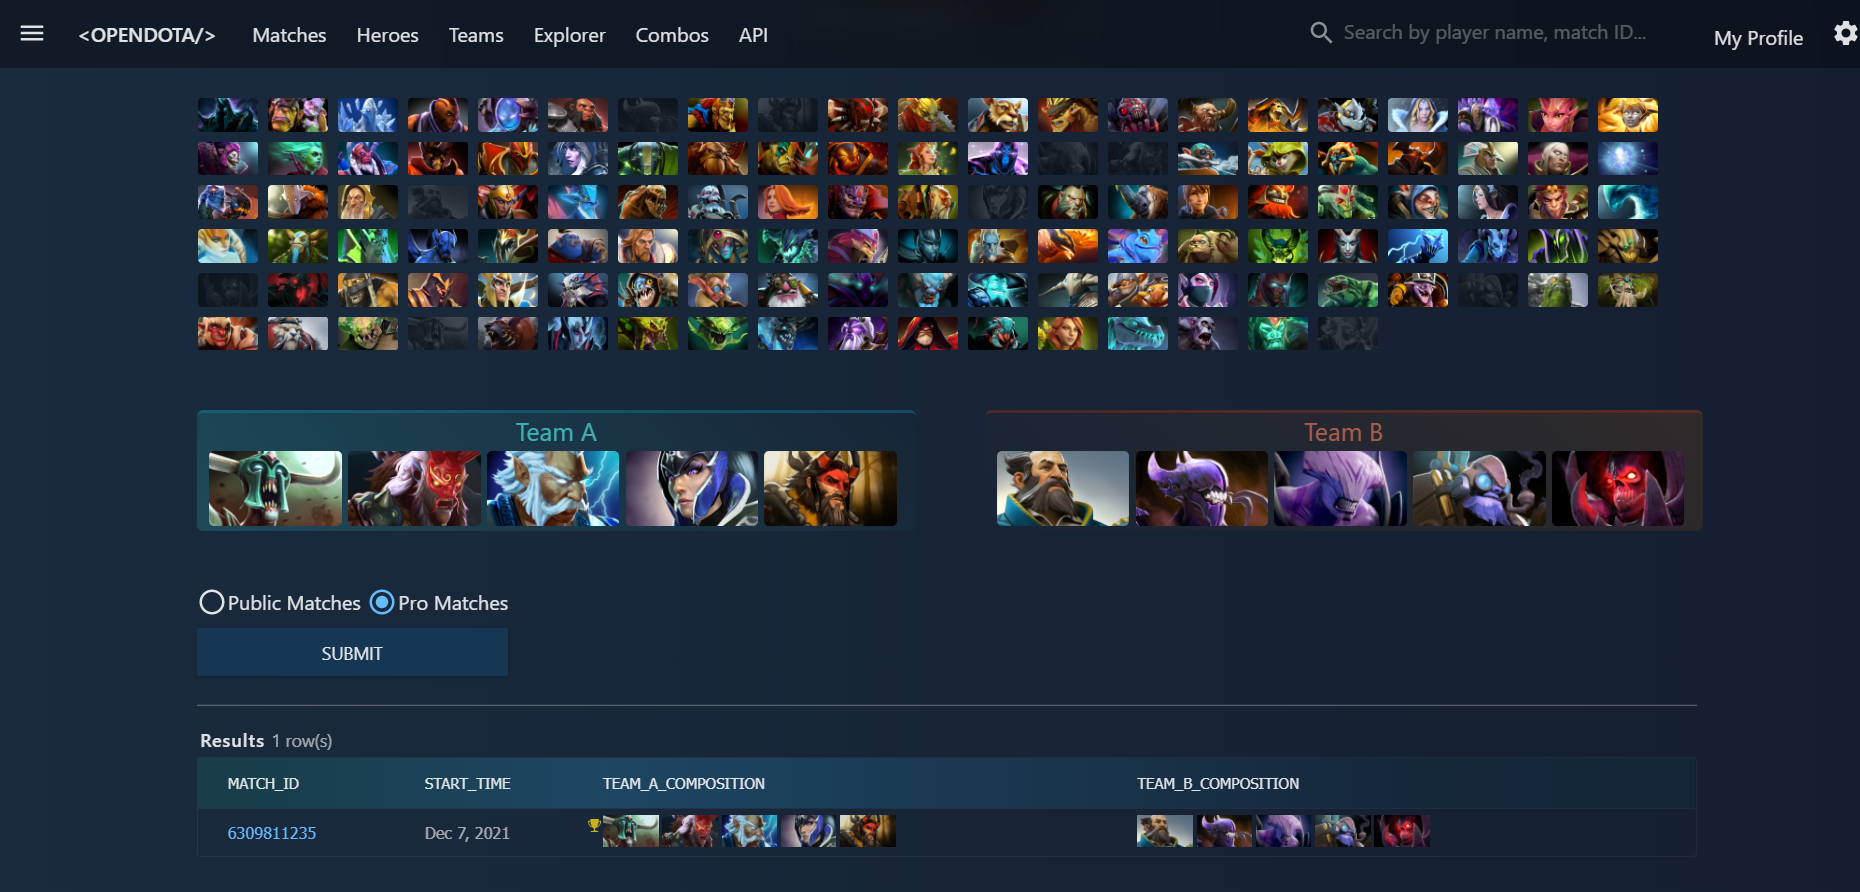
\includegraphics[width=.9\textwidth]{figures/dota1}
	\centering
	\caption{\LaTeX{} Na obrázku si vyberáme šampiónov pre oba tímy a následne nám vybehnú zápasy, ktoré prebehli s týmito podmienkami. \label{dota1}}
	
\end{figure}


 \begin{figure}[h!]
	
	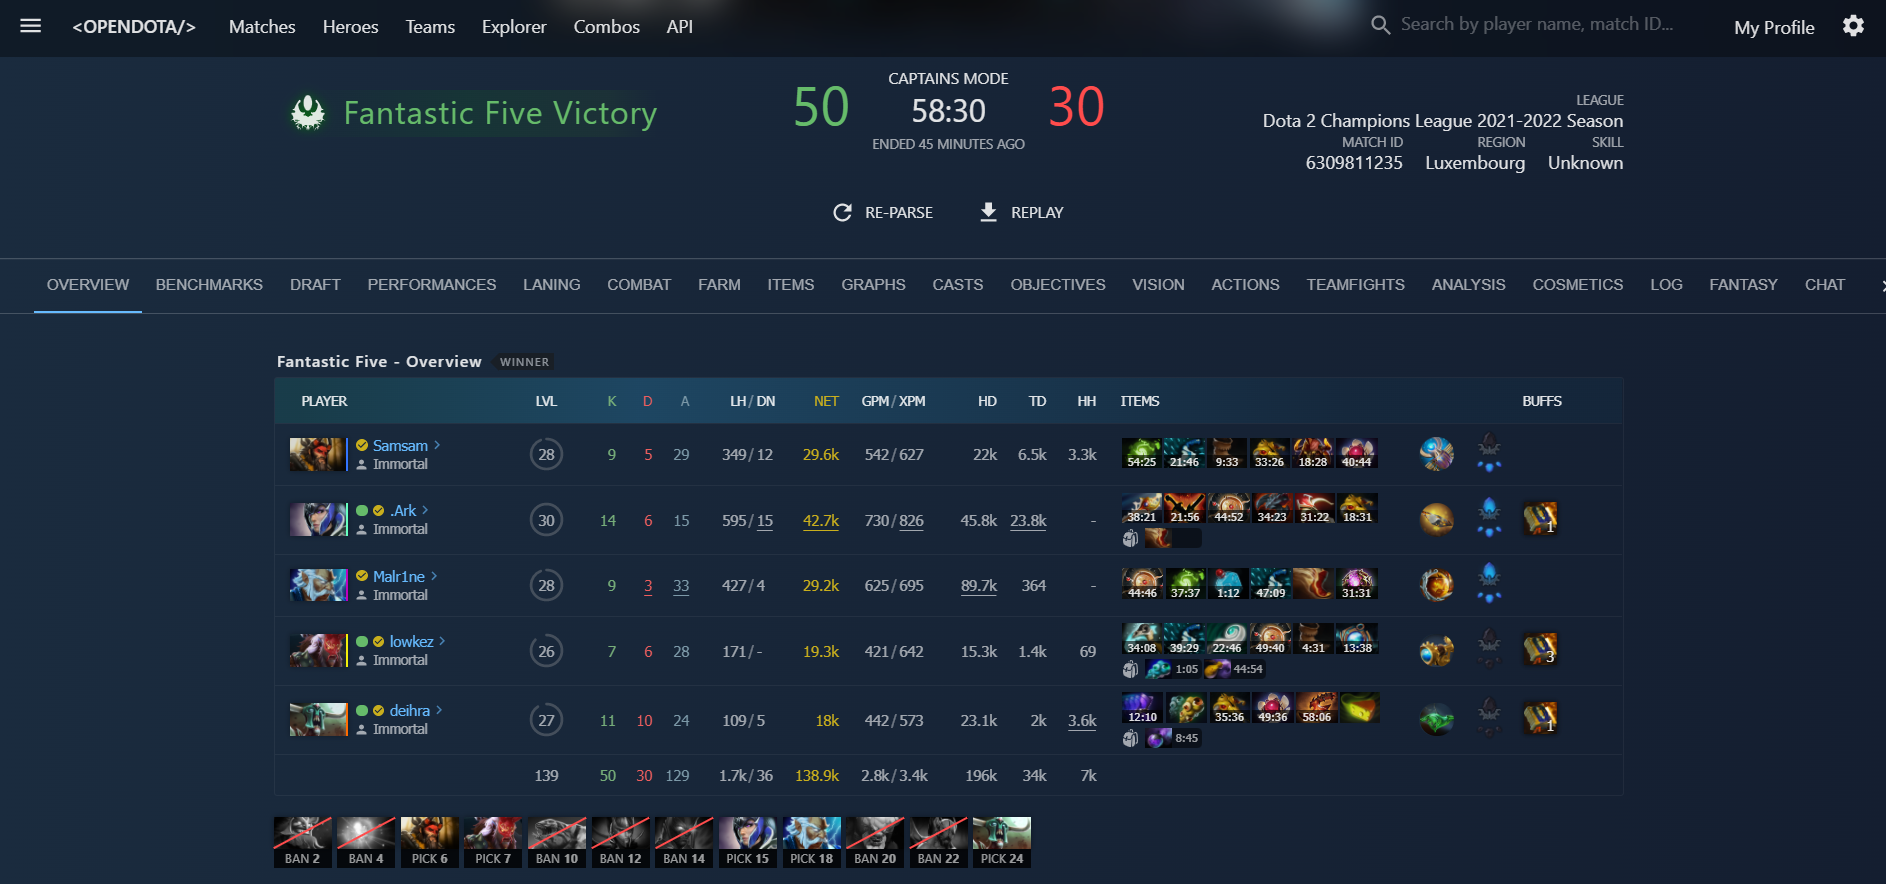
\includegraphics[width=.9\textwidth]{figures/dota2}
	\centering
	\caption{\LaTeX{} Po rozkliknutí zápasu si v zázname vieme pozrieť výhercu a všetky informácie sprevádzajúce daný zápas. \label{dota2}}
	
\end{figure}

\subsubsection{Dáta hry Dota 2}

match\_id - unikátne ID zápasu \\
duration - dĺžka zápasu \\
start\_time - začiatok zápasu \\
radiant\_team\_id - ID radiant tímu \\
radiant\_name - meno radiant tímu \\
dire\_team\_id - ID dire tímu \\
dire\_name - meno dire tímu \\
leagueid - ID ligy\\
league\_name - meno ligy\\
series\_id - ID série\\
series\_type - typ série\\
radiant\_score - skóre radiant\\
dire\_score - skóre direy\\
radiant\_win - výherca\\
name - meno hráča\\
radiant\_picks - radiant vybraní šampióni\\
radiant\_bans - radiant zabanovaní šampióni\\
dire\_picks - dire vybraní šampióni\\
dire\_bans - dire zabanovaní šampióni


\subsubsection{Vyhodnotenie hry Dota 2}
Znovu sa pozrieme na 3 oblasti. \\ \\ 
Publikum Doti a dosah je v porovnaní s CSGO nižší, na druhej strane jeho hráči sú odhodlaní brániť ju za každú cenu, čo môže mať negatívny, ale aj pozitívny efekt. Vzhľadom na  Potenciál/veľkosť publika a stávkovania. Efektívnosť využitia umelej inteligencie a dostupnosť, respektíve využiteľnosť dát z hier.
\\ \\
Dáta pri Dote môžeme rozdeliť na dve kategórie : 
\\ \\
1. Dáta na predpoveď pred vybratím šampiónov : \\
Tieto dáta sú obmedzené z dôvodu, že nevieme akých šampiónov budú dané dva tímy hrať. Takže sa spoliehame na predošlé výsledky daných dvoch tímov a ich stretnutí navzájom alebo s podobnými tímami. Takisto, ak sú noví hráči v tíme, vieme sa pozrieť aj na dáta individuálnych hráčov a na ich stretnutia z predošlých tímov. \\
Ďalšia podmienka, ktorou by sa dala predikcia vylepšiť, vychádza z porovnaní dát hráčov v danom tíme a šampiónov, ktorí sú práve v turnaji alebo v Patchi najviac hraní. Napríklad práve v rotácii najhranejších Carry šampiónov na profesionálnej scéne je daných 10 a týchto 10 porovnáme s hráčom v Carry pozícii, koľko má za nich nahraných profesionálnych hier alebo na ich SoloQ účte a ich výhernosť/gold per minute/KDA s týmito šampiónmi.  
\\ \\
2. Dáta na predpoveď po vybratí šampiónov : \\
Týchto dát je kvantum, lebo vieme použiť dáta o šampiónoch nie len z profesionálnych hier, ale aj z hier normálnych hráčov z vyšších líg v pomere hodnotenia, inak povedaného hodnotiaceho rebríčka. Vedeli by sme použiť dáta aj z nižšie postavených hráčov Doty, ale to by s vysokou pravdepodobnosťou zhoršilo výsledok predikcie vzhľadom na fakt, že hra top 80 percent hráčov a hra top 0.003 percent hráčov sa nedá porovnať. Veľmi dôležité informácie by teda boli o výkonnosti šampiónov ako gold per minute/average KDA alebo winrate. Zároveň by bolo veľmi zaujímavé skombinovať kompatibilnosť šampiónov spolu, spojením dvoch alebo viacerých šampiónov a ich spoločný priemerný winrate.


\subsection{League of Legends}
Liga Legiend je najrozšírenejšia MOBA hra na svete s viac ako 3 miliónmi každodenných používateľov a viac ako 100 miliónmi mesačných používateľov primárne z Číny. \cite{leaguefeed} 

 \begin{figure}[h!]
	
	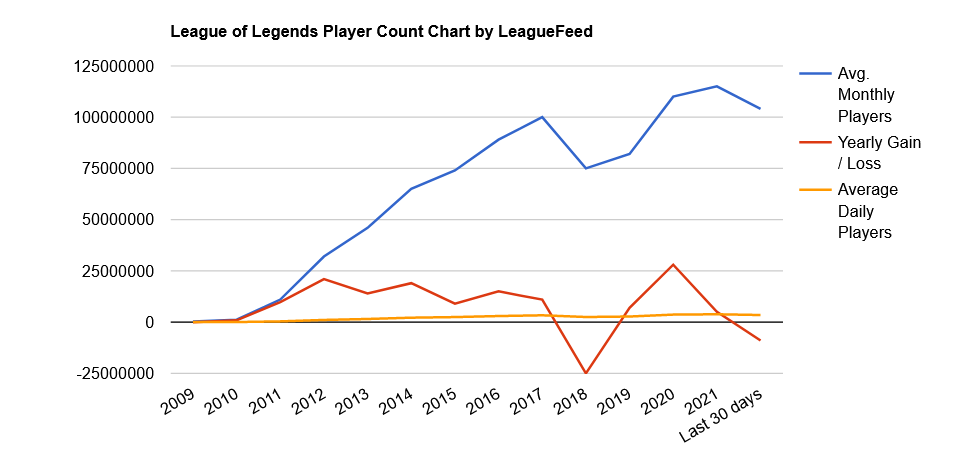
\includegraphics[width=.9\textwidth]{figures/leaguegraph}
	\centering
	\caption{\LaTeX{}   \label{leaguegraph}}
	
\end{figure}

Hra je z pohľadu tretej osoby a delí sa na dva tímy po piatich hráčoch. Víťazný tím je ten, ktorý zničí nepriateľskú základňu. Hráči zabíjaním nepriateľských minionov dostávajú peniaze, ktoré môžu využiť na zlepšenie ich výzbroje, čo im dá väčšiu šancu na zabitie nepriateľa a následne nepriateľskej základne.
\\ 
Riot games má podobne ako Dota verejne dostupné informácie pre developerov na stránke : 
\\ 
https://developer.riotgames.com/  
\\
a informácie o profesionálnych zápasoch na :
\\
https://lol.fandom.com/wiki/League\_Championship\_Series

\subsubsection{Dáta hry League of Legends}

date - dátum zápasu \\
blueteam - meno modrého tímu \\
redteam - meno červeného tímu \\
winner - víťaz \\
bluebans - bany modrého tímu \\
redbans - bany červeného tímu \\
bluepicks - vybraní šampióni modrého tímu \\
redpicks - vybraní šampióni červeného tímu \\
blueroster - hráči modrého tímu \\
redroster - hráči červeného tímu 

\subsubsection{Vyhodnotenie hry League of Legends}

Publikum z našich 3 hier ma LOL definitívne najväčšie, a to hlavne z dôvodu masívnej popularity v Číne, kde League of Legends má väčšiu popularitu a prestíž ako hocijaké iné, či už športy, hudba, tanec alebo spev. \cite{chinalol} 
\\
Aktuálne rozšírenie stávkovania na víťazný tím nie je vzhľadom na veľkosť publika až také rozšírené ako pri Dote a Lolku. To môže ovplyvňovať aj fakt, že gambling je v Číne vysoko ilegálny, až na výnimky ako mesto Macau.\cite{chinagambling}
\\
Využitie  umelej inteligencie v Lolku je veľké vzhľadom na verejne dostupné dáta a hlavne vysokú využiteľnosť.
\\
Dáta sú primárne veľmi podobné Dote, kde ich rozdeľujeme na dve časti, pred a po vybratí šampiónov.
\\
Veľmi lukratívne dáta, ktoré sú nanešťastie zatajené pred verejnosťou, sú dáta z hier, nazvané scrims. Pred oficiálnym začatím, napríklad svetového turnaja, sú všetky tímy zvolané a prítomné v usporiadajúcej krajine. Približne 3 týždne tieto tímy hrajú medzi sebou tréningové alebo kondičné zápasy, ktoré nie sú hodnotené, ale obsahujú veľa dôležitých informácií a taktík, ktoré tímy odskúšavajú. S prístupom k týmto dátam by sa dalo odskúšať veľa nových predikcií, ale k týmto dátam majú prístup len dané tímy a dáta sú vysoko chránené. Jedinou možnosťou, ako sa k nim dostať, by bol povolený prístup od tímov alebo odkúpenie za veľa peňazí.
\\


\section{Analýza dostupných spracovaní dát}
Časť analýzy dostupných spracovaní dát sa bude venovať jednotlivým druhom umelej inteligencie.

\subsection{Supervised learning}
Podkategória umelej inteligencie, ktorá používa daný dataset na natrénovanie modelu.

\subsection{Reinforcement learning}
Časť umelej inteligencie, pri ktorej sa sledujú kroky inteligentných agentov na maximalizáciu efektívnosti dosiahnutia cieľa.
